\section{Results}
Table \ref{main} presents our preferred CS estimators of overall ATT with and without controlling for county baseline characteristics. We notice that controlling for county baseline characteristics gives quite different estimates. Without controlling for county baseline characteristics, born after EBT leads to significantly higher WIC participation. But the positive impact is gone when controlling for baseline characteristics. When controlling for baseline characteristics, estimates of the impact of WIC on WIC participation of births given by LEUM or LEUM minority mothers remain significant and positive but their magnitudes become much larger. Figure \ref{cs_es} presents dynamic effects of EBT on WIC participation. We notice that controlling for county baseline characteristics smooths the pretrends, making estimates more convincing. As in Table \ref{main}, born after EBT significantly increases share of WIC births of LUEM mothers by 9.18\%, and by 14.82\% if mothers are also minority. We consider that the impacts are large for LEUM or LEUM minority mothers given the ATTs are larger than 10\% of dependent variable mean. Figure \ref{group_att} presents group-specific ATTs for all births, LEUM births, and LEUM minority births. Our overall ATTs are primarily driven by counties that implemented EBT in 2013 and 2019-2021. Estimates for 2019-2021 are less precise.


\begin{table}[!htbp] 
	\begin{center}
		\caption{\textsc{Impacts of WIC EBT on Share of WIC Births}} 
		\label{main} 
		\footnotesize 
		\begin{tabularx}{.9\linewidth}{@{}l*{6}{>{\centering\arraybackslash}X}@{}}
			\\[-1.8ex]\hline 
			\hline 
			\\[-1.8ex] 
			& \multicolumn{6}{c}{WIC Birth Ratio} \\ 
			\cline{2-7}   
			\\[-1.8ex] & \multicolumn{2}{c}{All Births} & \multicolumn{2}{c}{LEUM Births} & \multicolumn{2}{c}{\scriptsize LEUM $\times$ Black/Hisp.} \\ 
			\\[-1.8ex] & \multicolumn{1}{c}{(1)} & \multicolumn{1}{c}{(2)}& \multicolumn{1}{c}{(3)} & \multicolumn{1}{c}{(4)} & \multicolumn{1}{c}{(5)} & \multicolumn{1}{c}{(6)} \\ 
			\hline \\[-1.8ex] 
			Born after EBT   &0.0082$^{*}$ & -0.0154 & 0.0239$^{***}$ & 0.0918$^{**}$ & 0.0229$^{**}$ & 0.1482$^{**}$\\
			& (0.0043) & (0.0229) & (0.0089) & (0.039) & (0.0124) & (0.0657)\\ 
			& & & & & & \\
			Baseline Characteristics  & & \checkmark & & \checkmark &  & \checkmark\\
			Observations   & 21,047 & 20,956  & 7,722 & 7,709 & 3,549 & 3,549\\
			Dep. Var. Mean (DVM)  & 0.4316 &0.4321 & 0.7362 & 0.7363 & 0.7415 & 0.7415 \\
			\%(ATT/DVM)  & 1.90\% & -3.56\%  & 3.25\% & 12.47\% & 3.09\% & 19.99\%\\
			\hline \\[-1.8ex] 
			\hline 
			\hline \\ [-5.0ex] 
		\end{tabularx}
	\end{center}
	\footnotesize
	\vspace{4pt}
	\vspace{4pt}
	Notes: LEUM refers to births given by unmarried mothers with less than high school education. Regressions are weighted by the number of births of cells. Standard errors are clustered at the county level. We use not-yet-treated counties as comparison group. We drop cells with fewer than 25 births. $^{***}$, $^{**}$, and $^{*}$ indicate that the estimates are significant at the 1\%, 5\%, and 10\% levels.
\end{table} 

\begin{figure}[!htbp]
	\begin{subfigure}[t]{.325\textwidth}
		\centering
		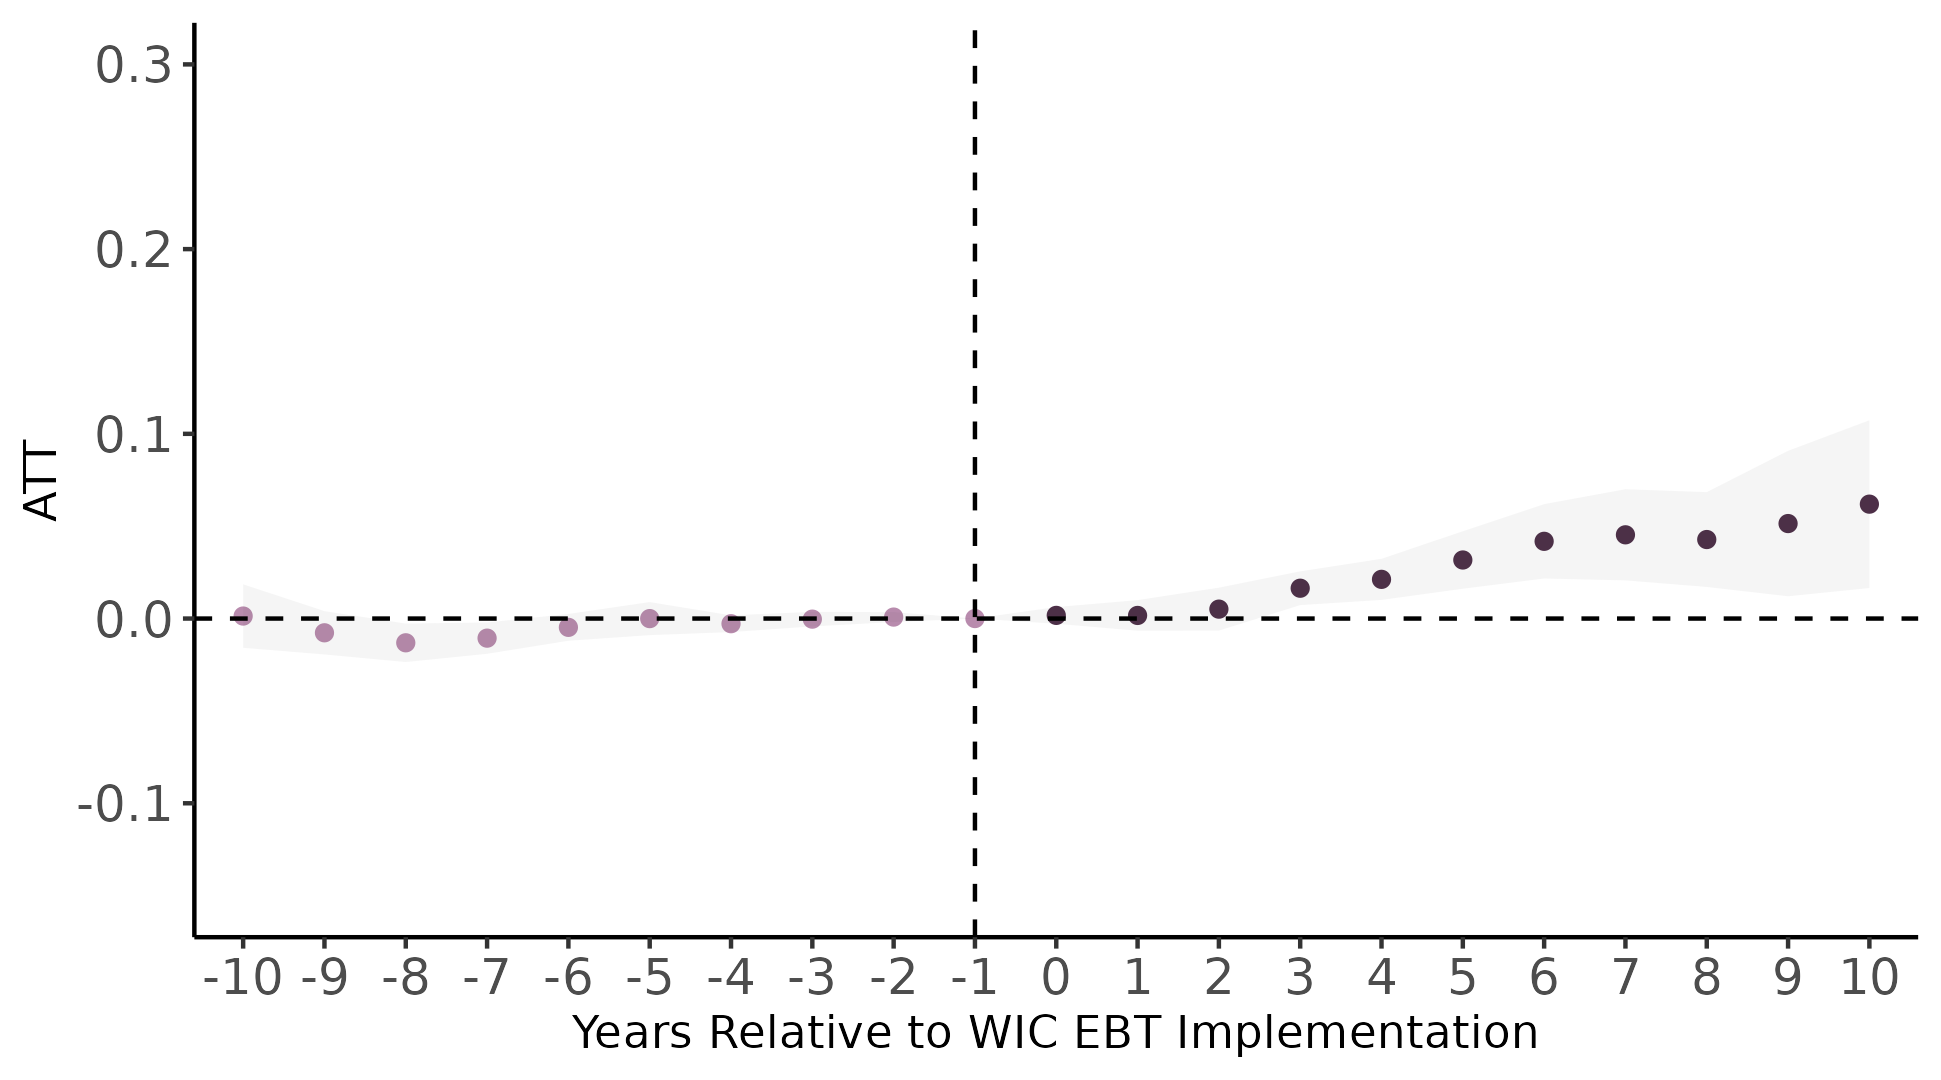
\includegraphics[width=\textwidth]{wic_br_dyn_all_noncov.png}  
		\caption{All births, without Controlling for County Baseline Characteristics}
		\label{cs_es1}
	\end{subfigure}
	\begin{subfigure}[t]{.325\textwidth}
		\centering
		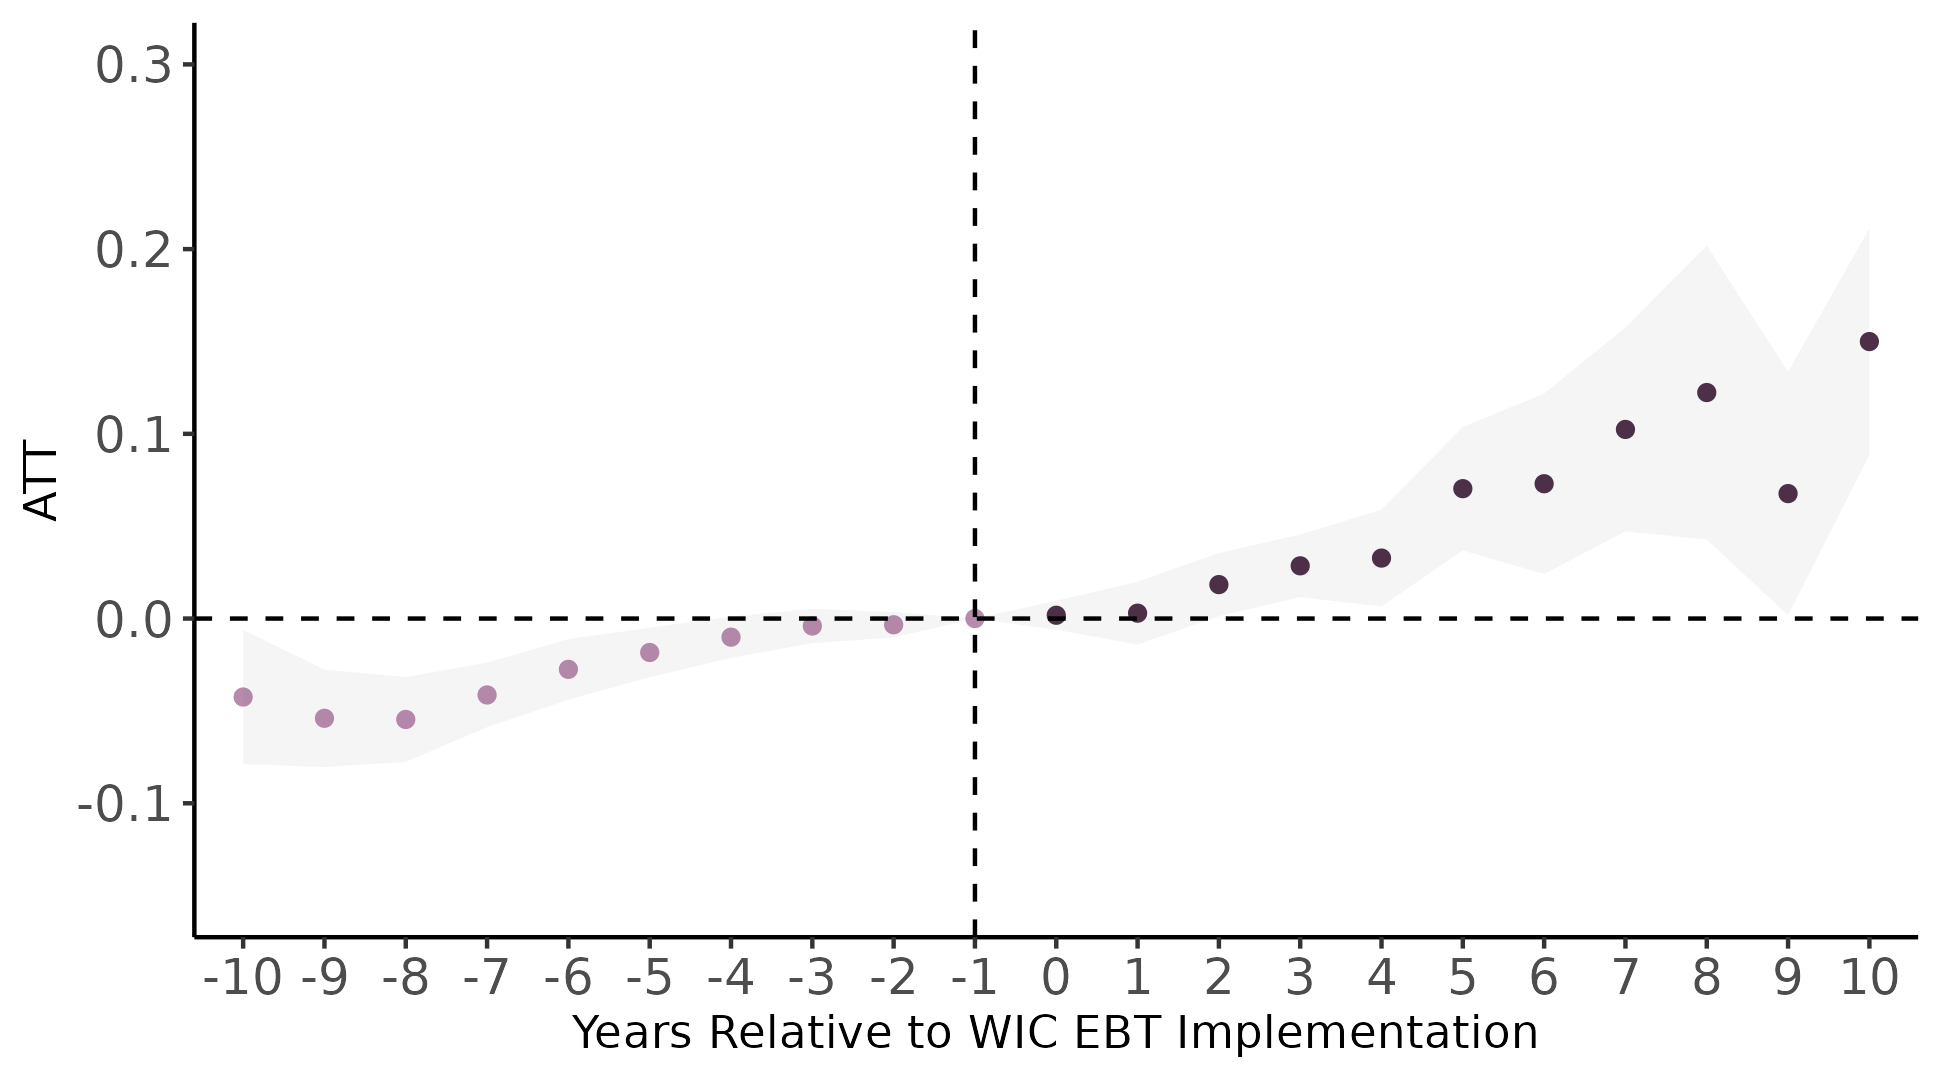
\includegraphics[width=\textwidth]{wic_br_dyn_leum_noncov.png}  
		\caption{LEUM Births, without Controlling for County Baseline Characteristics}
		\label{cs_es2}
	\end{subfigure}
	\begin{subfigure}[t]{.325\textwidth}
		\centering
		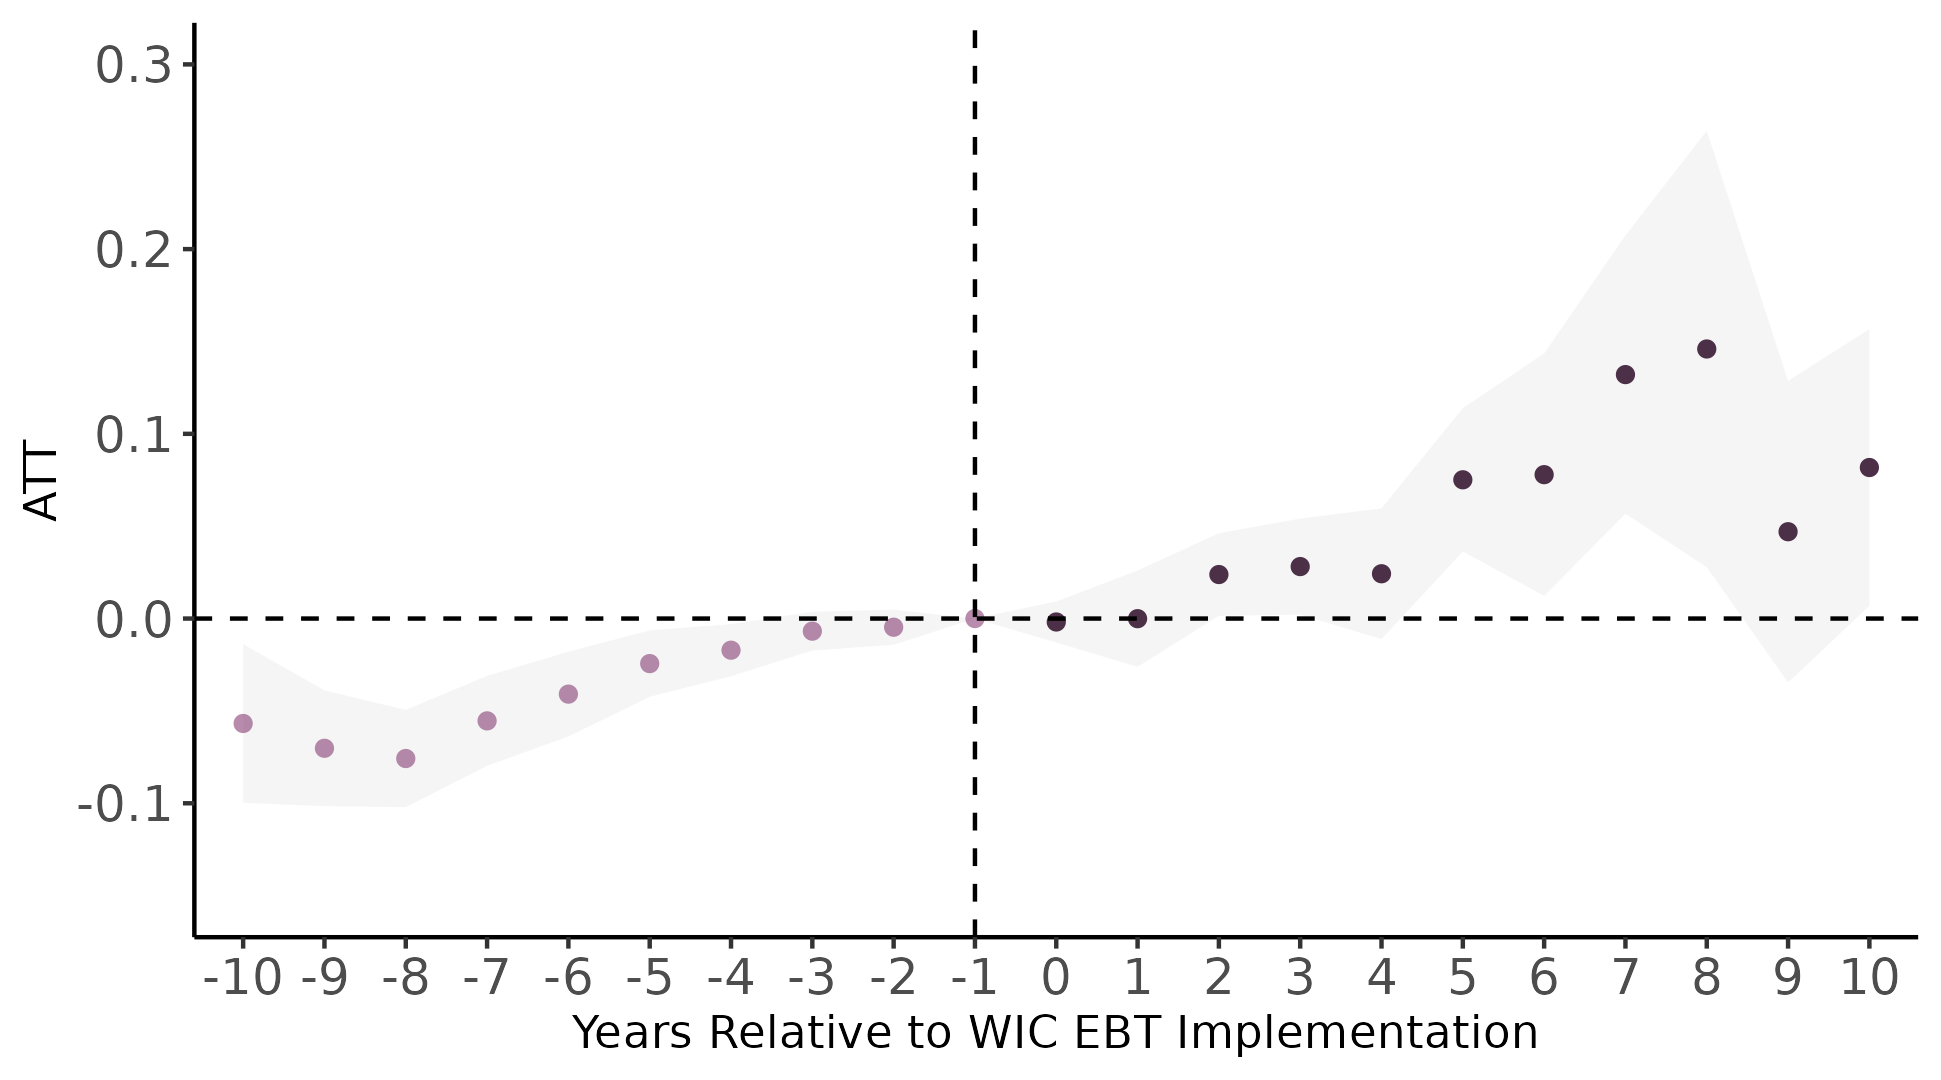
\includegraphics[width=\textwidth]{wic_br_dyn_leum_minor_noncov.png}  
		\caption{LEUM $\times$ Black/Hispanic, without Controlling for County Baseline Characteristics}
		\label{cs_es3}
	\end{subfigure}
	\begin{subfigure}[t]{.325\textwidth}
		\centering
		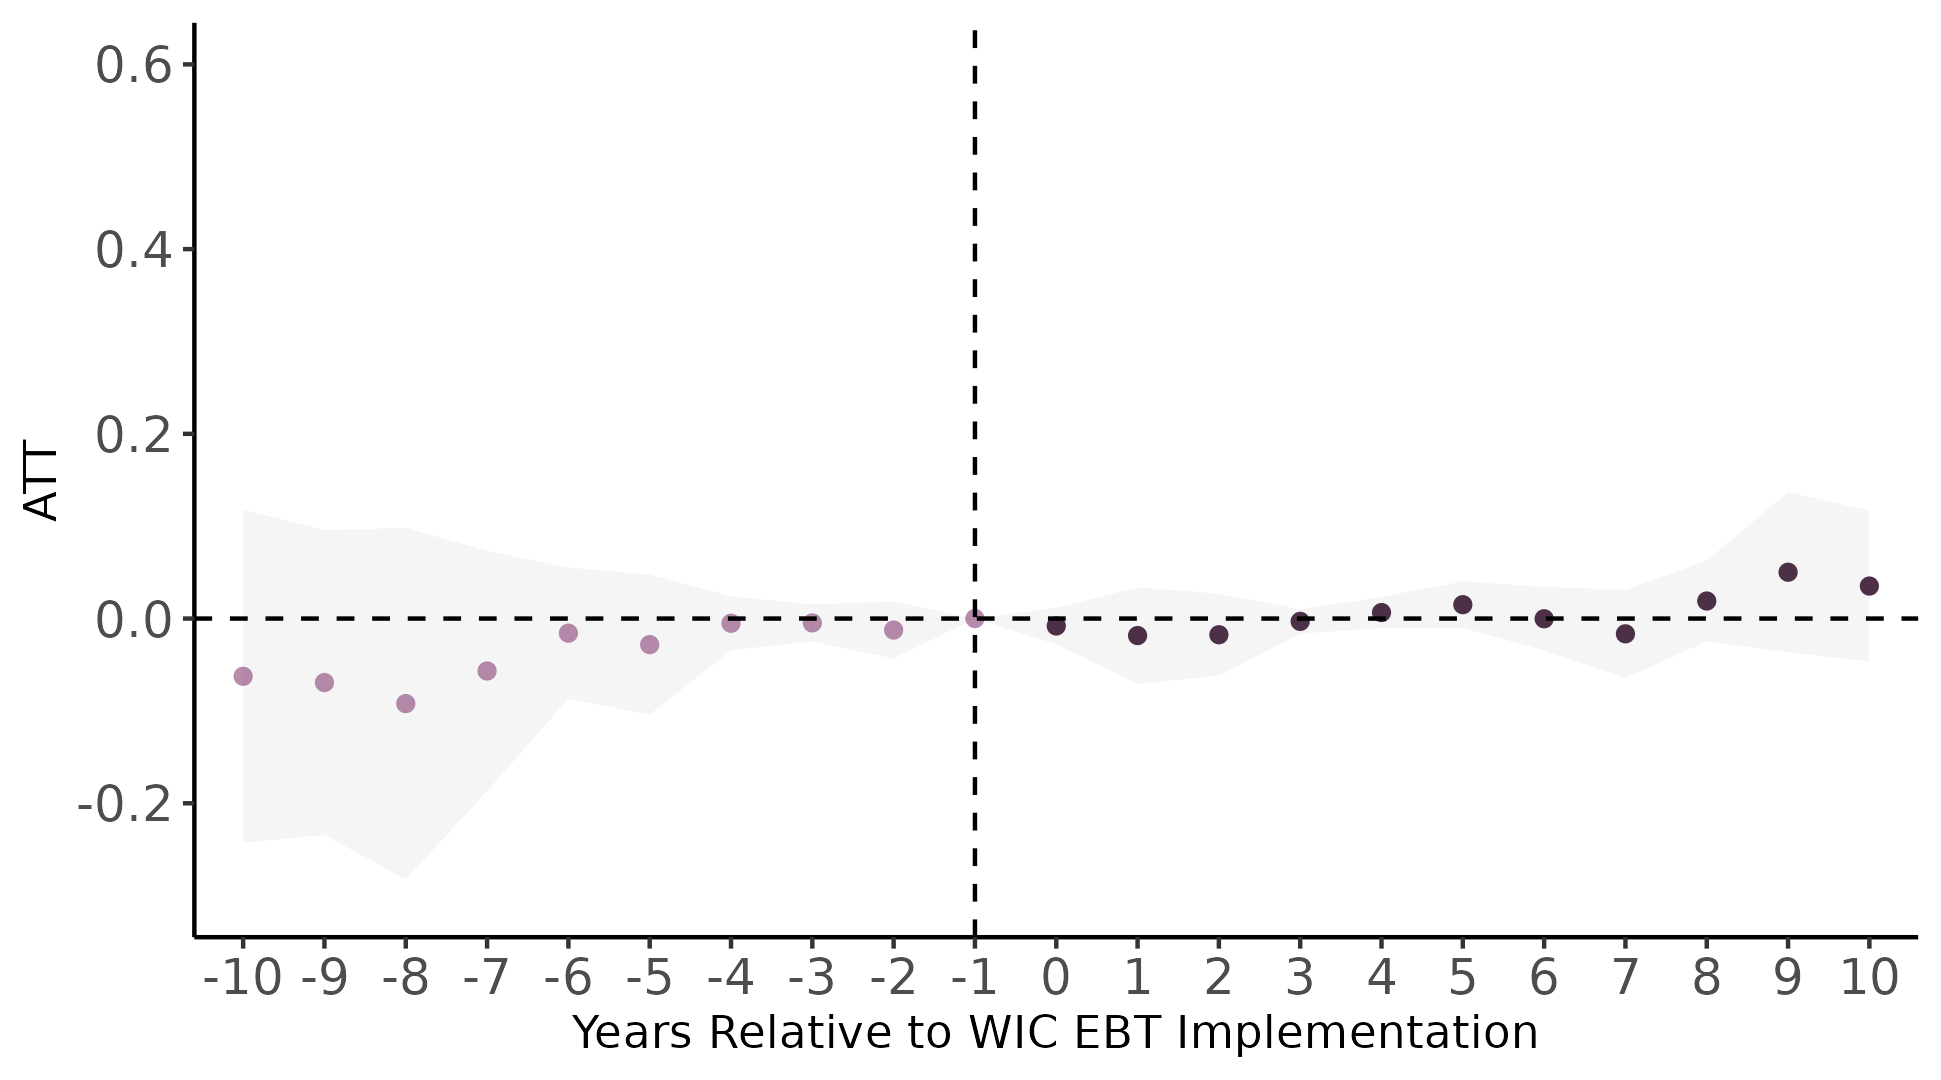
\includegraphics[width=\textwidth]{wic_br_dyn_all.png}  
		\caption{All Births, with Controlling for County Baseline Characteristics}
		\label{cs_es1}
	\end{subfigure}
	\begin{subfigure}[t]{.325\textwidth}
		\centering
		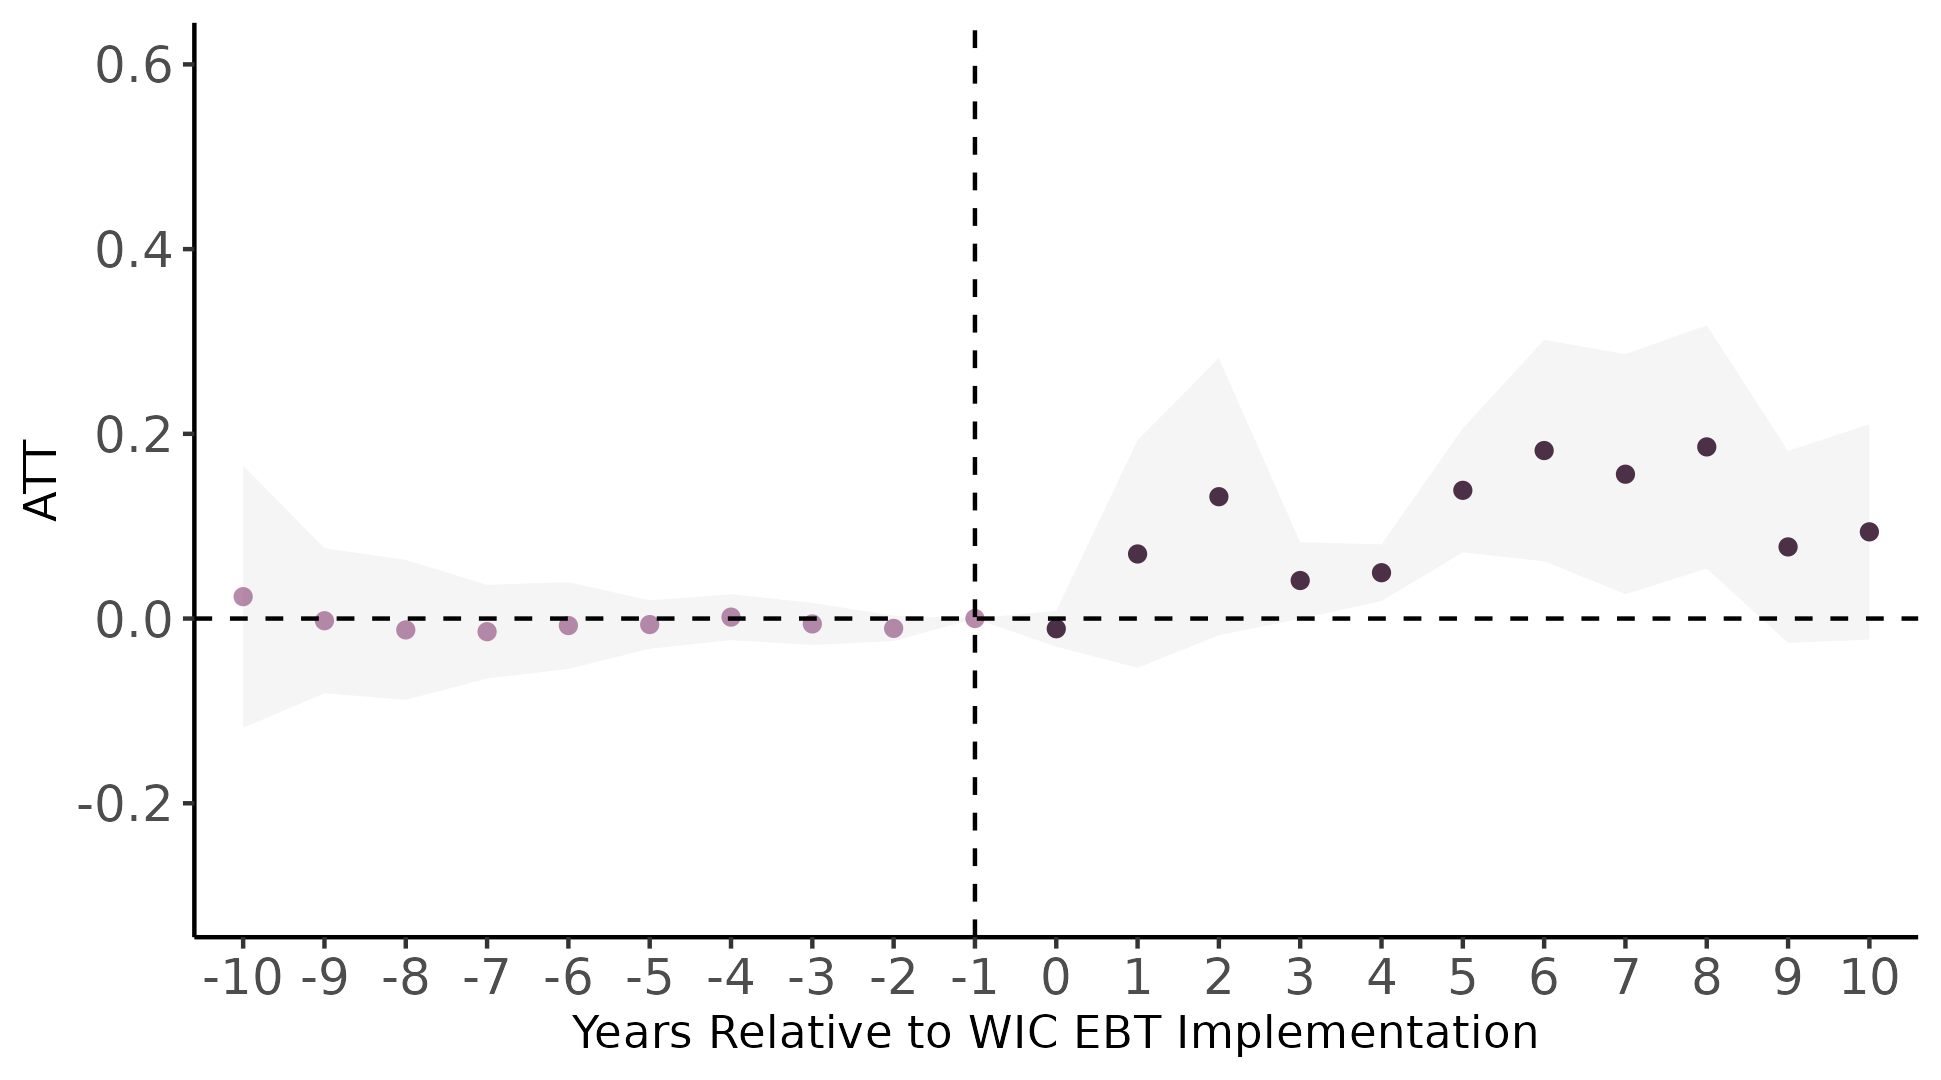
\includegraphics[width=\textwidth]{wic_br_dyn_leum.png}  
		\caption{LEUM Births, with Controlling for County Baseline Characteristics}
		\label{cs_es2}
	\end{subfigure}
	\begin{subfigure}[t]{.325\textwidth}
		\centering
		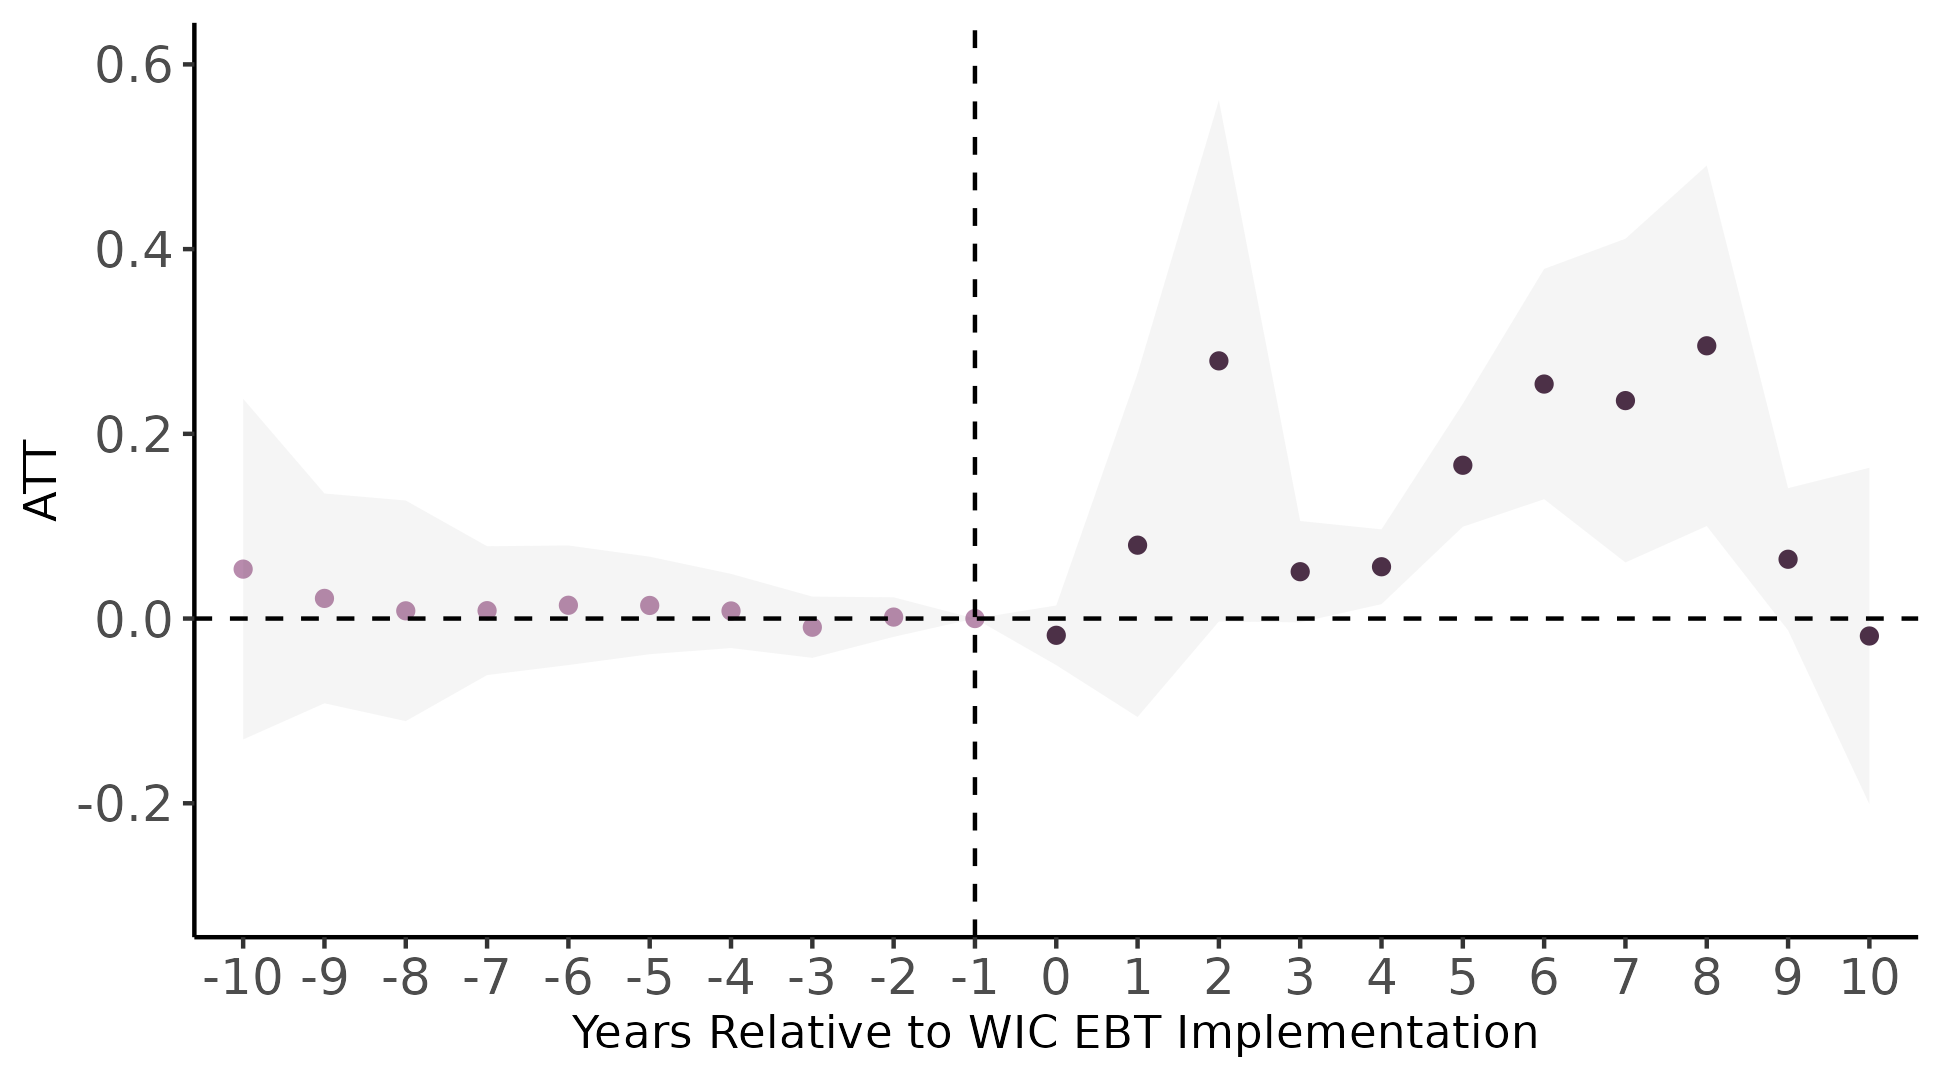
\includegraphics[width=\textwidth]{wic_br_dyn_leum_minor.png}  
		\caption{LEUM $\times$ Black/Hispanic, with Controlling for County Baseline Characteristics}
		\label{cs_es3}
	\end{subfigure}
	\caption{\textsc{Dynamic Effects of WIC EBT on Share of WIC Births}}
	\label{cs_es}
	\footnotesize
	\vspace{6pt}
	\vspace{4pt}
	Notes: LEUM refers to births given by unmarried mothers with less than high school education. Regressions are weighted by the number of births of cells. Standard errors are clustered at the county level. We use not-yet-treated counties as comparison group. We drop cells with fewer than 25 births.
\end{figure}

\begin{figure}
	\begin{center}
		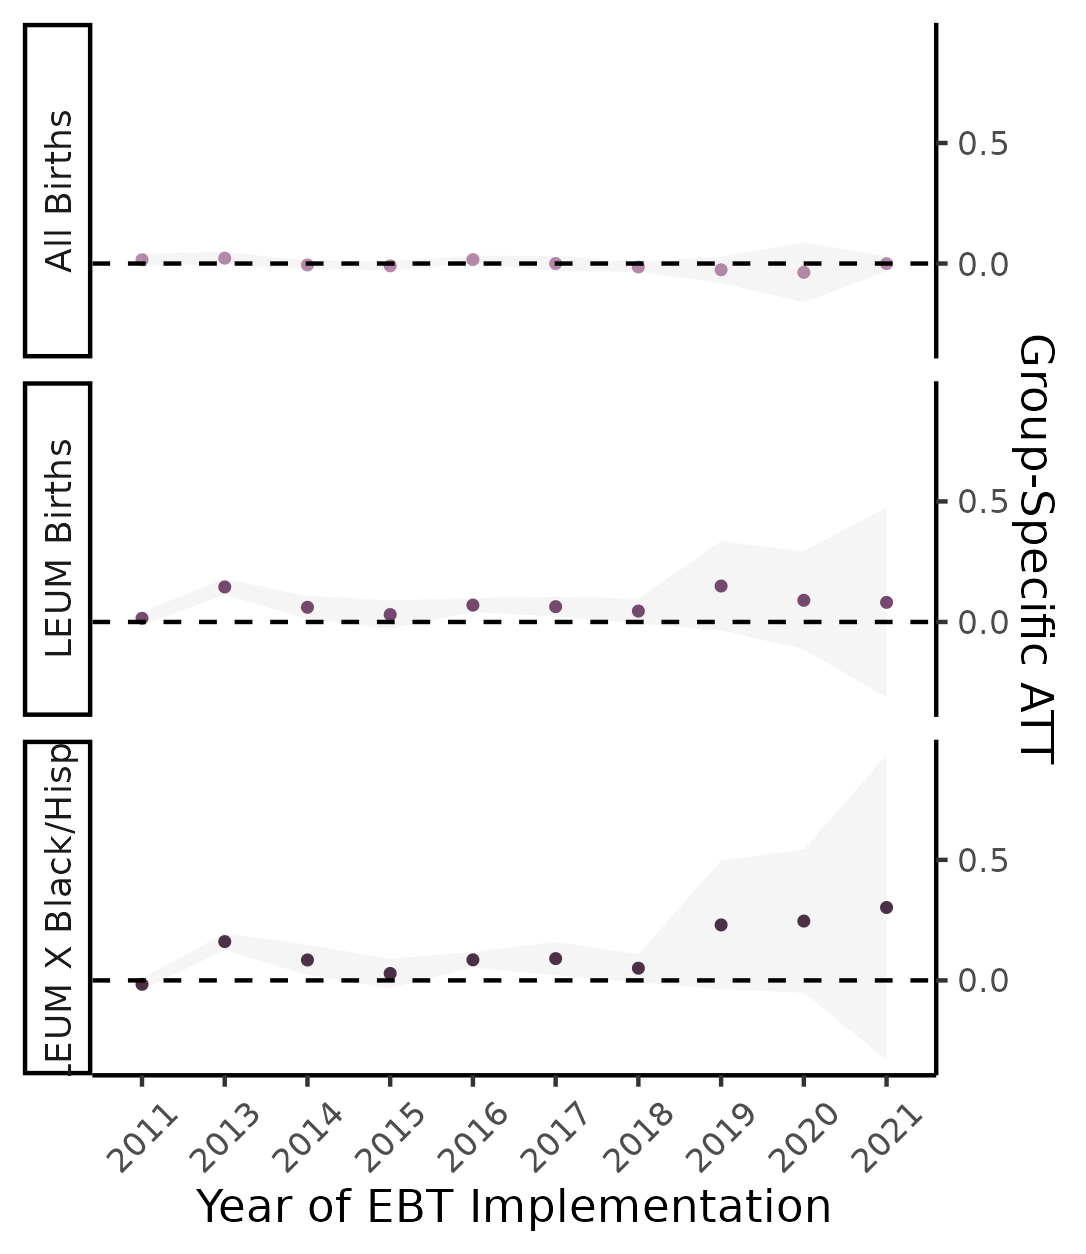
\includegraphics[width=.6\textwidth]{group_att.png}  
		\caption{\textsc{Group-specific Effects of WIC EBT on WIC Birth Ratio}}
		\label{group_att}
	\end{center}
	\footnotesize
	Notes: 
\end{figure}

\section{Robustness}

\begin{table}[!htbp]
	\begin{center}
		\caption{\textsc{Sensitivity to Sample Selection}} 
		\label{} 
		\scriptsize
		\begin{tabularx}{\linewidth}{@{}l*{9}{>{\centering\arraybackslash}X}@{}}
			\\[-1.8ex]\hline 
			\hline 
			\\[-1.8ex] 
			& \multicolumn{9}{c}{WIC Birth Ratio} \\ 
			\cline{2-10} \\
			& \multicolumn{3}{c}{All} & \multicolumn{3}{c}{LEUM} & \multicolumn{3}{c}{LEUM $\times$ Black/Hisp.} \\
			\cmidrule(lr){2-4}\cmidrule(lr){5-7} \cmidrule(lr){8-10}
			& Full    & $\geq 15$     & $\geq 35$     & Full    & $\geq 15$     & $\geq 35$    & Full    & $\geq 15$     & $\geq 35$     \\
			[1ex]            & (1)     & (2)      & (3)    & (4)  & (5)     & (6)      & (7)    & (8) & (9)    \\
			\midrule
			Born after EBT  & -0.0077 & -0.0167 & -0.0143 & 0.0447 & 0.0853$^{**}$  &0.1085$^{**}$ & 0.0152 & 0.1378$^{**}$  & 0.1673$^{**}$ \\
			& (0.0167) & (0.0198) & (0.0226) & (0.0317) & (0.0380) & (0.0475) & (0.0569) & (0.0515) & (0.1113)\\  \\
			Covariates     & \checkmark & \checkmark & \checkmark & \checkmark & \checkmark & \checkmark
			& \checkmark & \checkmark & \checkmark  \\
			Observations    & 28,756 & 22,438 & 19,955 & 19,864 & 10,153 & 6,110 & 11,466 & 4,420  & 3,016\\
			Dep. Var. Mean (DVM) & 0.4215 & 0.4261 & 0.4358 & 0.7393 & 0.7390 & 0.7319 & 0.7482 & 0.7440 & 0.7366\\
			\%(ATT/DVM) & 1.83\% & 3.92\% & 3.28\% & 6.05\% & 12.65\% & 14.82\% & 2.03\% & 18.52\% & 22.71\%\\
			\hline \\[-1.8ex] 
			\hline 
			\hline \\ [-5.0ex] 		
		\end{tabularx}
	\end{center}
	\footnotesize
	\vspace{4pt}
	Notes: 
\end{table}

\begin{table}[!htbp] 
	\begin{center}
		\caption{\textsc{Two-way-fixed-effect Estimators and Goodman-Bacon Decomposition}} 
		\label{twfe} 
		\scriptsize 
		\begin{tabularx}{.75\linewidth}{@{}l*{3}{>{\centering\arraybackslash}X}@{}}
			\\[-1.8ex]\hline 
			\hline 
			\\[-1.8ex] 
			& \multicolumn{3}{c}{WIC Birth Ratio} \\ 
			\cline{2-4}   
			\\[-1.8ex] & All Births   & LUEM Births & LUEM $\times$ Black/Hisp.  \\ 
			\\[-1.8ex] & \multicolumn{1}{c}{(1)} & \multicolumn{1}{c}{(2)}  & \multicolumn{1}{c}{(3)} \\ 
			\hline \\[-1.8ex] 
			TWFE Est. &  0.0071$^{***}$  & 0.0099$^{***}$ & 0.0094$^{**}$  \\
			& (0.0013)& (0.0028) & (0.0043) \\ 
			TWFE Est., No Forbidden Comparison &  	
			0.0094 & 0.0181 & 0.0167 \\
			$\Delta$ after excl. the Forbidden Comparison &  	
			$\uparrow$ 32.39\% & $\uparrow$ 82.83\% &  $\uparrow$ 77.66\% \\
			& & & \\
			County FE & \checkmark & \checkmark & \checkmark \\
			Year FE & \checkmark & \checkmark & \checkmark  \\
			Observations & 18,824 & 7,709 & 3,549 \\
			Dep. Var. Mean & 0.4212 & 0.7363 & 0.7415 \\
			\hline \\[-1.8ex] 
			\hline 
			\hline \\ [-5.0ex] 
		\end{tabularx} 
	\end{center}
	\footnotesize
	Note: We use the same balanced panel as CS estimators. Goodman-Bacon decomposition can only work on balanced panels and can only identify the forbidden comparison (the later v.s. earlier group) for the case without any controls \citep{goodman2021difference}.
\end{table} 

\begin{table}[!htbp] 
	\begin{center}
		\caption{\textsc{Alternative Staggered DD Estimators}} 
		\label{sa} 
		\footnotesize 
		\begin{tabularx}{.9\linewidth}{@{}l*{6}{>{\centering\arraybackslash}X}@{}}
			\\[-1.8ex]\hline 
			\hline 
			\\[-1.8ex] 
			& \multicolumn{3}{c}{CS 2020} & \multicolumn{3}{c}{SA 2021}\\ 
			& \multicolumn{3}{c}{Last-treated as Comparison} & \multicolumn{3}{c}{}\\ 
			\cmidrule(lr){2-4}\cmidrule(lr){5-7} 
			& All Births & LEUM Births & LEUM $\times$ Black/Hisp. & All Births & LEUM Births & LEUM $\times$ Black/Hisp.\\ 
			\\[-1.8ex] & \multicolumn{1}{c}{(1)} & \multicolumn{1}{c}{(2)}& \multicolumn{1}{c}{(3)} & \multicolumn{1}{c}{(4)} & \multicolumn{1}{c}{(5)}& \multicolumn{1}{c}{(6)} \\ 
			\hline \\[-1.8ex] 
			Born after EBT   & -0.0269 & 0.1415$^{**}$ &0.1895$^{***}$ & 0.0078 & 0.0246$^{**}$ & 0.0256$^{**}$ \\
			& (0.0256) & (0.0614) &(0.0936) & (0.0054) &(0.0109) & (0.0141) \\
			& & & & & & \\
			Covariates  & \checkmark & \checkmark & \checkmark & \checkmark & \checkmark & \checkmark \\
			Observations    & 20,956 & 7,709 & 3,549 & 20,955 &7,708 & 3,548 \\
			Dep. Var. Mean   & 0.4321 & 0.7363 & 0.7415 & 0.4321 &0.7363 & 0.7415 \\
			\%(ATT/DVM)  & -6.23\% & 19.22\% & 25.56\% & 1.81\% & 3.34\% & 3.32\% \\
			\hline \\[-1.8ex] 
			\hline 
			\hline \\ [-5.0ex] 
		\end{tabularx}
	\end{center}
	\footnotesize
	\vspace{4pt}
	Notes: SA 2021 estimators are from \cite{sun2021estimating}.
\end{table} 


\begin{table}[!htbp] 
	\begin{center}
		\caption{\textsc{Alternative Definitions of Likely Eligible Sub-population}} 
		\label{sa} 
		\footnotesize 
		\begin{tabularx}{\linewidth}{@{}l*{6}{>{\centering\arraybackslash}X}@{}}
			\\[-1.8ex]\hline 
			\hline 
			\\[-1.8ex] 
			& Age $\leq$ 22 & Education $<$ HS & Unmarried & Black/Hispanic & LEUM Births & LEUM $\times$ Black/Hisp.\\ 
			\\[-1.8ex] & \multicolumn{1}{c}{(1)} & \multicolumn{1}{c}{(2)}& \multicolumn{1}{c}{(3)} & \multicolumn{1}{c}{(4)} & \multicolumn{1}{c}{(5)}& \multicolumn{1}{c}{(6)} \\ 
			\hline \\[-1.8ex] 
			Born after EBT   & -0.0269 & 0.1415$^{**}$ &0.1895$^{***}$ & 0.0078 & 0.0246$^{**}$ & 0.0256$^{**}$ \\
			& (0.0256) & (0.0614) &(0.0936) & (0.0054) &(0.0109) & (0.0141) \\
			& & & & & & \\
			Covariates  & \checkmark & \checkmark & \checkmark & \checkmark & \checkmark & \checkmark \\
			Observations    & 20,956 & 7,709 & 3,549 & 20,955 &7,708 & 3,548 \\
			Dep. Var. Mean   & 0.4321 & 0.7363 & 0.7415 & 0.4321 &0.7363 & 0.7415 \\
			\%(ATT/DVM)  & -6.23\% & 19.22\% & 25.56\% & 1.81\% & 3.34\% & 3.32\% \\
			\hline \\[-1.8ex] 
			\hline 
			\hline \\ [-5.0ex] 
		\end{tabularx}
	\end{center}
	\footnotesize
	\vspace{4pt}
	Notes: SA 2021 estimators are from \cite{sun2021estimating}.
\end{table} 


\begin{table}[!htbp] 
	\begin{center}
		\caption{\textsc{Composition Change}} 
		\label{sa} 
		\footnotesize 
		\begin{tabularx}{.6\linewidth}{@{}l*{2}{>{\centering\arraybackslash}X}@{}}
			\\[-1.8ex]\hline 
			\hline 
			\\[-1.8ex] & \multicolumn{1}{c}{Share of LEUM} & \multicolumn{1}{c}{Share of LEUM} \\
			& \multicolumn{1}{c}{Births} & \multicolumn{1}{c}{$\times$ Black/Hisp.} \\
			\\[-1.8ex] & \multicolumn{1}{c}{(1)} & \multicolumn{1}{c}{(2)}\\ 
			\hline \\[-1.8ex] 
			Born after EBT   & 0.0032 & 0.0062$^{*}$\\
			& (0.0037) & (0.0035)  \\
			& &  \\
			Covariates  &\checkmark & \checkmark  \\
			Observations   & 20,956 & 20,956  \\
			Dep. Var. Mean   & 0.0906 & 0.0319  \\
			\%(ATT/DVM)  & 3.53\% & 19.44\%  \\
			\hline \\[-1.8ex] 
			\hline 
			\hline \\ [-5.0ex] 
		\end{tabularx}
	\end{center}
	\footnotesize
	\vspace{4pt}
	Notes: LEUM births refer to the births of unmarried mothers who do not graduate from high school (LEUM: less educated and unmarried). Advantaged births are those given to high-school-graduated, married, white mothers. Standard errors of both estimators are clustered at the county level. We drop cells with fewer than 25 births. $^{***}$, $^{**}$, and $^{*}$ indicate that the estimates are significant at the 1\%, 5\%, and 10\% levels.
\end{table} 
